\documentclass[twocolumn]{aastex62}

\newcommand{\vdag}{(v)^\dagger}
\newcommand\aastex{AAS\TeX}
\newcommand\latex{La\TeX}
\usepackage{amsmath}
\usepackage{physics}
\usepackage{hyperref}
\usepackage{natbib}
\usepackage[T1]{fontenc}
\usepackage[english]{babel}
\usepackage[utf8]{inputenc}
\usepackage{wasysym}

\begin{document}

\title{\Large AST5220-Milestone II: The Universes Opacity}

\author{Nils-Ole Stutzer}

\begin{abstract}
    
    \textit{The codes for this paper can be found at:} \newline \url{https://github.com/SagittariusA-Star/AST5220-Milestones}
\end{abstract}

\section{Introduction} \label{sec:Intro}

\section{Method} \label{sec:Method}

\section{Results/Discussion}\label{sec:Results}

\begin{figure*}
    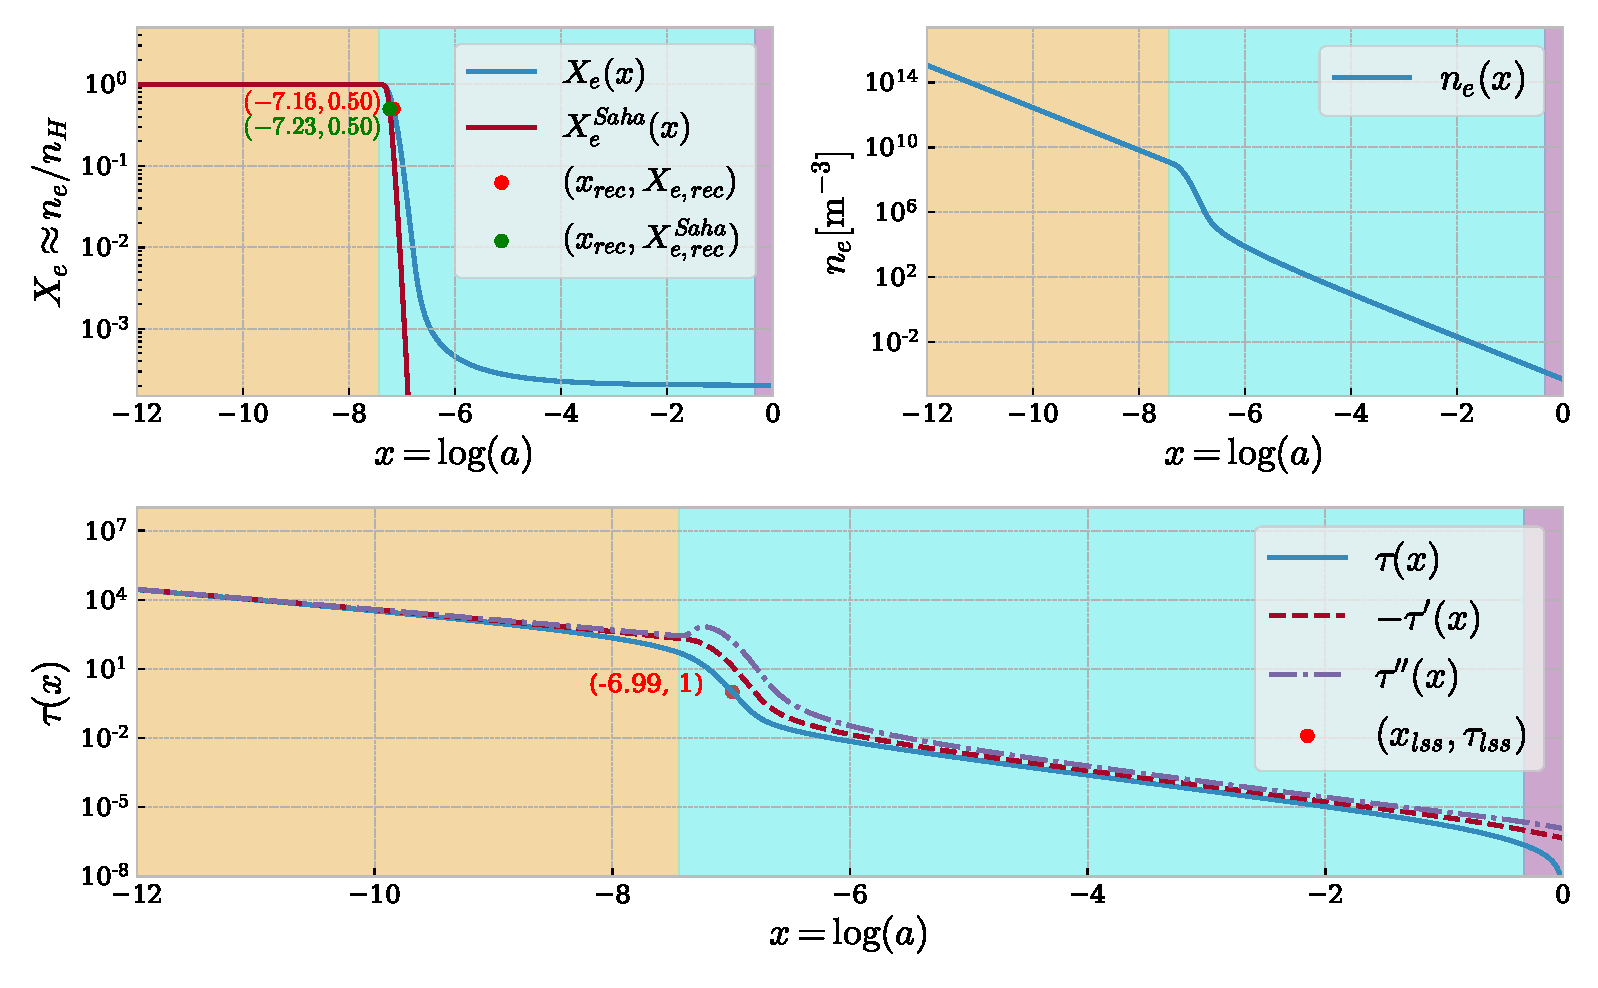
\includegraphics[scale = 0.65]{Figures/Xe_ne_tau.pdf}
    \caption{\textbf{Upper left}: Figure showing the free electron fraction $X_e$ 
    as a function of the log-scale factor $x$. \textbf{Upper right}: Figure showing the free electron density $n_e$
    as a function of the log-scale factor $x$. \textbf{Lower panel}: Figure showing the optical depth $\tau(x)$ of the universe due to 
    Thomson scattering on free electrons only, as well at the derivative $\tau'(x)$ and second oder derivative $\tau''(x)$ w.r.t 
    and as functions of the log-scale factor $x$. \textbf{Note}: The background color in all the plots shows the epoch of dominance
    for reference. Yellow markes the era of radiation dominance, blue the epoch of matter domination
    and purple corresponds to the epoch of dark energy. The color domain is found by checking 
    when the corresponding density parameter is dominant,
    however, in reality the transitions between each epoch should be smoother than shown.}
    \label{fig:Xe}
\end{figure*}

\begin{figure*}
    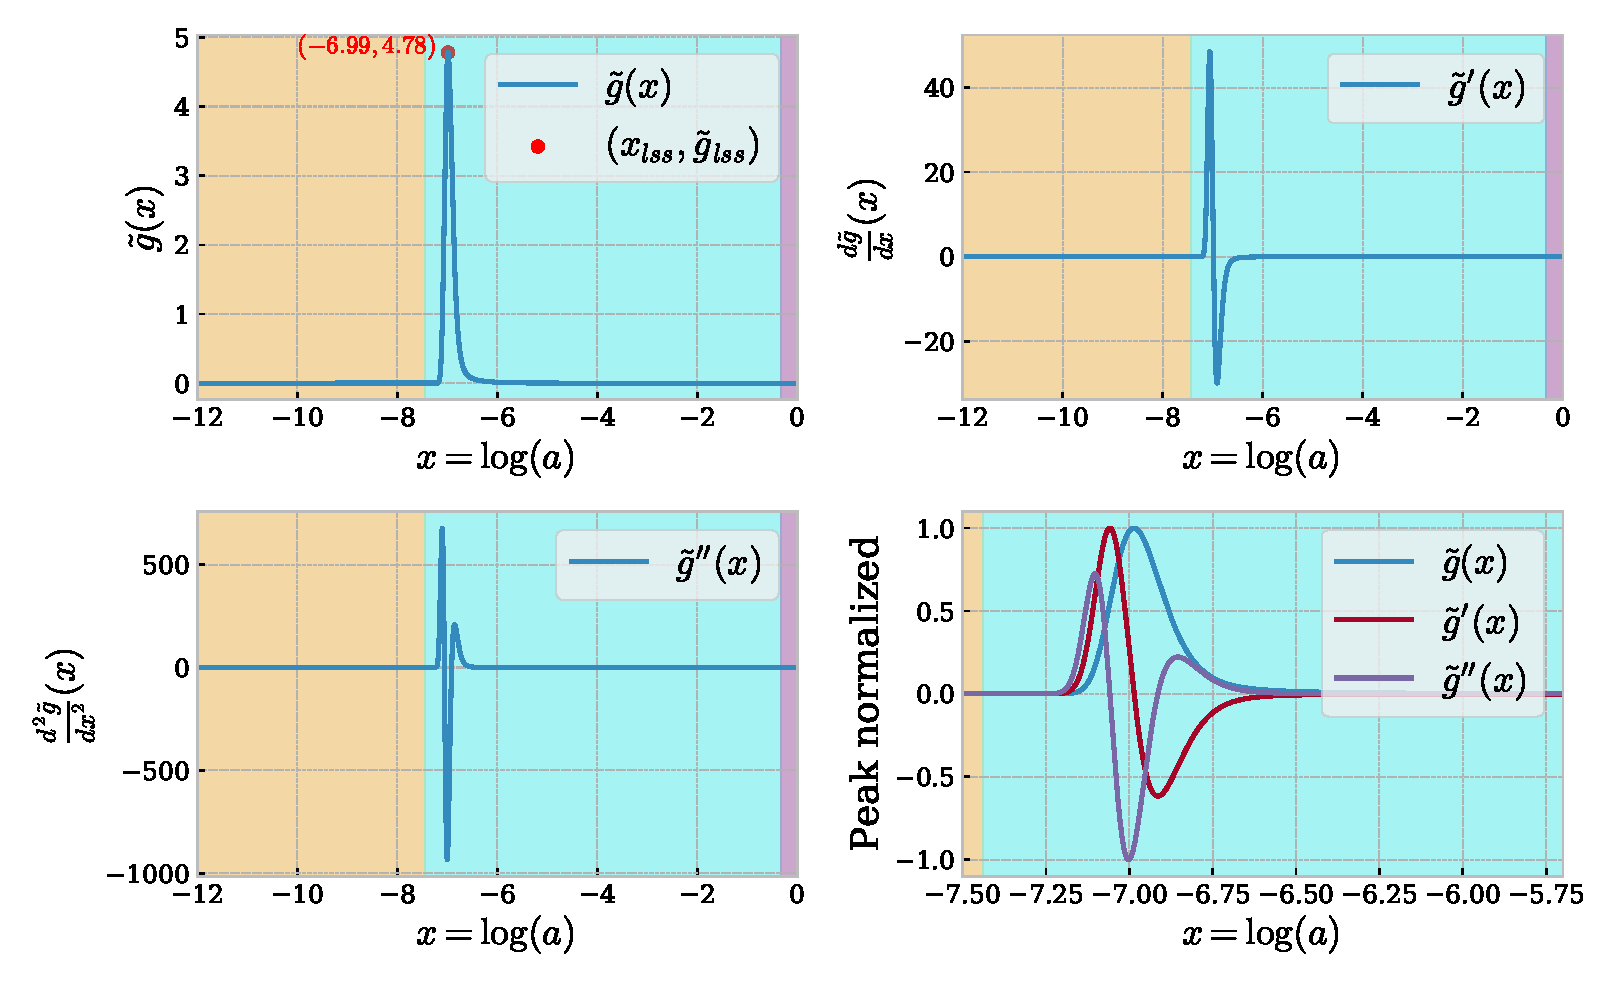
\includegraphics[scale = 0.65]{Figures/g_tilde.pdf}
    \caption{\textbf{Upper left}: Figure showing the un-normalized visibility function $\tilde{g}$ as a function of the log-scale factor $x$.
    The red dot markes the peak of $\tilde{g}$ 
    and its $x$ value corresponds to the log scale factor of the surface of last scattering. 
    \textbf{Upper right}: Figure showing the un-normalized first order derivative of $\tilde{g}$ w.r.t. and as a function of the log-scale factor. 
    \textbf{Lower left}: Figure showing the un-normalized second order derivative of $\tilde{g}$ w.r.t. and as a function of the log-scale factor.
    }
    \label{fig:g_tilde}
\end{figure*}

\section{Conclusion} \label{sec:Conclusion}


\bibliography{ref}
\bibliographystyle{aasjournal}
\end{document}